\chapter{Methodology and System Design}
\label{chap:met}

\section{Navigation}

% Our research goal is to create a system that would classify an incoming question as simple or requiring human processing, then answer the simple questions fully autonomously, and help the expert to answer the second kind of questions faster. In this chapter, we are presenting the approach we used to achieve this goal. In Section 3.2 we describe our research design - what methods we use and how we implemented our product. In Section 3.-3. we talk about data - how we collected, prepared, and analyzed them. In Section 3.*-3.* we describe step by step the implementation.

Our research goal is to create a system that would classify an incoming question as standardized or complex (see Chapter \ref{chap:intro}), then answer the standardized questions fully autonomously and assist an expert to answer the complex questions. This system is called \textit{Automatic Learner Support (ALS)}. Furthermore, we are going to integrate the ALS system into the NamazApp e-learning application \cite{namazapp}. NamazApp is a mobile application that helps Muslims learn how to perform \textit{namaz} - Islamic worship or prayer \cite{merriamwebster2025}. The application has Q\&A section where users can ask any questions related to Islam or the app itself. Before integrating the ALS the questions have been answered manually by the expert (NamazApp founder). The general design of the system with the existing NamazApp components is presented in Section \ref{sec:system_design}. Then the two components that we develop are described: Knowledge Base (Section \ref{sec:knowledge_base_design}) and ALS (Section \ref{sec:als_design}).

\section{General System design}
\label{sec:system_design}

In this section, we describe the architecture and internal components of the whole system including the NamazApp client application, backend, database, knowledge base, ALS. Fig. \ref{fig:architecture-diagram} illustrates the conceptual architecture, showing how the components (internal modules, external resources, and user-facing interfaces) interact with each other. Our design follows an AI-in-the-loop paradigm, in which LLM-based automation handles simple recurring queries, while more complex or nuanced questions are delegated to human operators. 
The system comprises three main layers:
\begin{enumerate}
    \item Client layer
    \begin{itemize}
        \item Learner (end user): The individual who submits questions to the support chat in the app.
        \item NamazApp Operator (human support staff): The person responsible for monitoring automated responses and manually handling complex or novel queries. For simplicity, NamazApp operator is the expert that answers questions.
    \end{itemize}
    \item Business layer
    \begin{itemize}
        \item NamazApp Backend: it orchestrates message flow, interacts with the ALS module and with the Knowledge Base. 
        \item Automatic Learner Support module: RAG pipeline that interacts with LLM, NamazApp Backend, and the Knowledge base (via the Backend) and generates answers.
    \end{itemize}
    \item Data layer
    \begin{itemize}
        \item Knowledge Base: A repository of domain-specific documents and previously answered questions (PAQs). This knowledge base is vectorized to enable semantic search for retrieval augmented generation (RAG). It consists of two major parts: PAQ database and IslamQA database. They are described in Section \ref{sec:knowledge_base_design}.
        \item Support Databases: Other databases (e.g., for user profiles or application logs) that support the overall NamazApp infrastructure.
    \end{itemize}
\end{enumerate}

\begin{figure}
    \centering 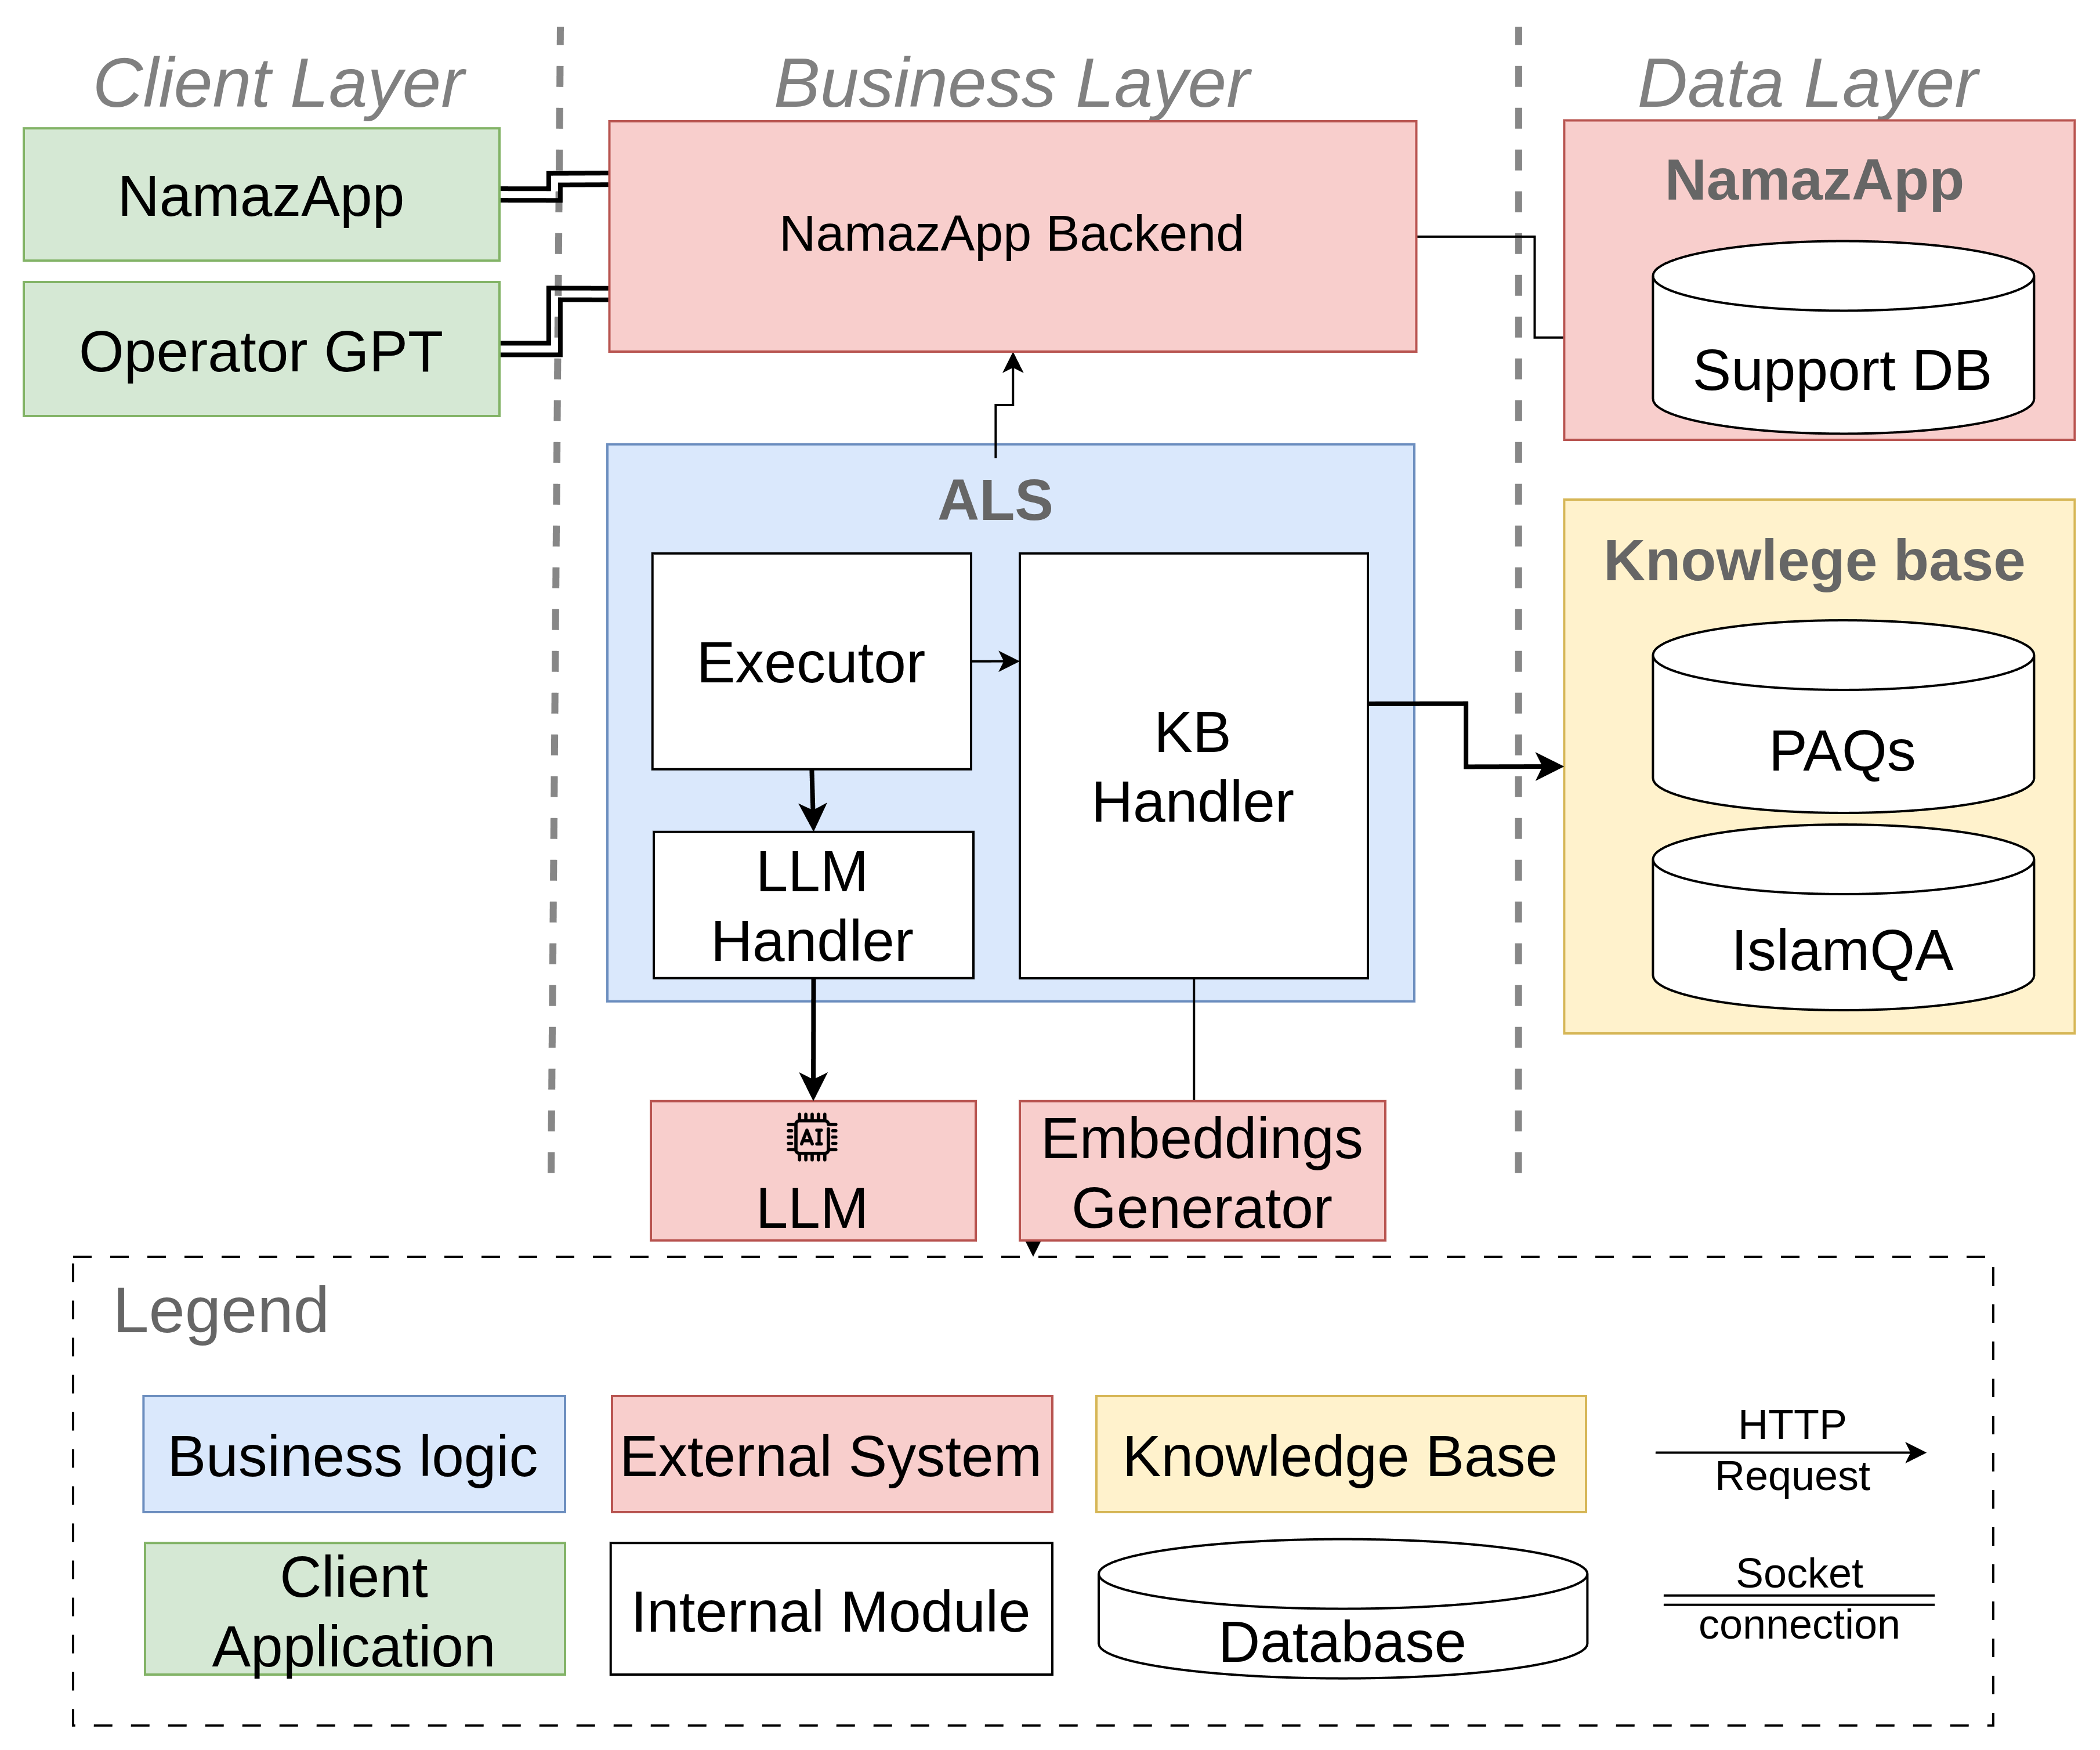
\includegraphics[width=0.5\linewidth]{figs/architecture.png}
    \caption{Architecture}
    \label{fig:architecture-diagram}
\end{figure}


\section{Knowledge Base design}
\label{sec:knowledge_base_design}

As we said, the Knowledge Base consists of two major components: PAQ database and IslamQA database.

\subsection{Previously Answered Questions (PAQ) database}

PAQ database is a vector database that contains previously answered questions (PAQs) from the NamazApp exclusively. All questions from NamazApp users that have been answered manually by the expert are stored here with the corresponding embedding vectors. This database is frozen, meaning that the new answered questions are not going to it. This was made intentionally for proper evaluation of results. 

The PAQ database is filled with data and managed by NamazApp developers, not by us, we just exploit it to retrievee most relevant questions and answers. The ALS system receives data from the database via NamazApp Backend. It has an endpoint that for a given question returns the most similar PAQs. Fig. \ref{fig:paq_db} presents the example response from the database (useless fields are omitted). The field \textit{"similarity"} is a float number that shows how similar the PAQ is to the given question. It is a cosine similarity between embedding vectors. The score 1 means that they are identical.

\begin{figure}[H]
    \centering
    \begin{minipage}{0.9\textwidth}
        \ttfamily
        \begin{verbatim}
{
    "id": 347,
    "question": "Can you make wuduh in the sink?",
    "answer": "Yes, you can make wudu (ablution) in the sink as long as 
        the water is clean and you wash all the necessary parts.",
    "similarity": 0.650584754452365
}
        \end{verbatim}
    \end{minipage}
    \caption{Example response from the PAQ database}
    \label{fig:paq_db}
\end{figure}

\subsection{IslamQA database}

Despite having the PAQ database, we decided to create another database from trustworthy sources to overcome the limitation of small amount of PAQs. Since we lacked the expertise to tell reliable information from unreliable, we turned to the experts at Darul-Ifta Tatarstan for guidance. They provided us with reliable information in various formats, including electronic books and encyclopedias covering topics like animal sacrifice, marriage, fasting, and charity. In addition, they recommended trustworthy websites, such as Annisa-today and Askimam, where we could explore answers to a wide range of questions organized by topic. 

So, IslamQA contains preprocessed data from these sources with embeddings. This database will be used in addition to the PAQ database.


\section{ALS design}
\label{sec:als_design}

Automatic Learner Support (ALS) system is a naive RAG pipeline \cite{gao2024retrievalaugmentedgenerationlargelanguage} that performs sequential actions. 
We developed the pipeline iteratively; overall we created three versions. Fig.~\ref{fig:pipeline-flow-v1} presents the high-level flow of the first version of the pipeline, in the second version the question extraction stage was improved, and in Fig. \ref{fig:pipeline-flow} you can observe the high-level flow of the last version of the pipeline. We added to it the integration with IslamQA database.

\begin{figure}
    \centering
    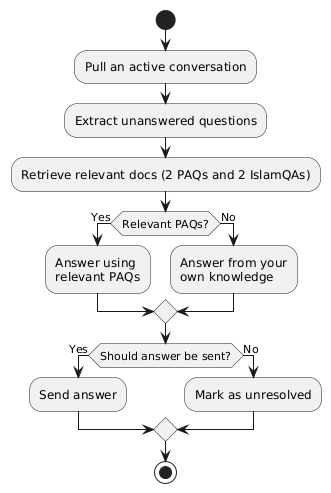
\includegraphics[width=0.5\linewidth]{figs/pipeline_flow_v1.png}
    \caption{The flow of the RAG pipeline V1 and V2: a high-level overview of system functionality}
    \label{fig:pipeline-flow-v1}
\end{figure}

\begin{figure}
    \centering
    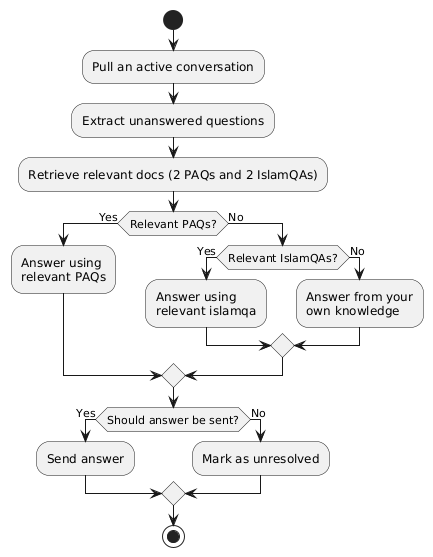
\includegraphics[width=0.5\linewidth]{figs/pipeline_flow.png}
    \caption{The flow of the RAG pipeline V3: a high-level overview of system functionality}
    \label{fig:pipeline-flow}
\end{figure}

Instead of processing questions, we work with conversations. This is made for the sake of convenience of collecting the results. \textit{A conversation} is a dialogue between a user and the NamazApp operator. A conversation might contain anything, but we are mainly interested in the \textit{salam} (Islamic greeting) because we have to reply to it and the questions the user asked. Moreover, some questions in a conversation could already be answered, in such a case the ALS should not answer it again. The ALS system's goal is to correctly extract unreciprocated salam and unanswered questions from a conversation, generate the answer to the question, and decide if the answer should be sent to the user.

As we mentioned earlier, we follow the AI-in-the-loop paradigm, so we process conversations in a loop. Each conversation is processed by the pipeline.

% TODO - refactor.
\textit{An active conversation} is a conversation in which the last message is from the user and that has not been marked as resolved. Active conversations are pulled from the NamazApp database, then the ALS extracts unanswered questions and unreciprocated salam. Furthermore, for each question it retrieves relevant PAQs and if they are present, generates the answer and sends to the user. The last version of the pipeline also uses IslamQA database along with the PAQs. It was added to address the limitation of small size of the PAQs database. Otherwise, it generates the answer not based on any PAQs (or IslamQA fatwas) and does not send it to the user. We describe the working flow and its implementation in Chapter~\ref{chap:impl}. 

\section{Conclusion}

Our goal is to create an ALS system and integrate it with the NamazApp e-learning platform. Based on the PAQ database, our RAG pipeline should extract unanswered questions from the active conversations, retrieve revelant PAQs, generate the answer, and send it if appropriate.




% \section{Research design}

% Dar-ul-Ifta in Tatarstan already works for the 5 years. They usually receive a question through an email or a phone call. They answer around 380 questions per month, which is 95 per week approximately.
% To make their work more efficient, we introduce our LLM-based agent system.

% First of all, we collaborated with an employee of Darul-Ifta in Tatarstan as our customer and domain expert. We conducted requirements elicitation. 
% Secondly, we collected and prepared a database of fatwas from different sources. See Section \ref{sec:data} for more details.
% Thirdly, we delivered a simple MVP (see Section \ref{sec:mvp1}) for the customer to use as a part of our requirements engineering process.
% Then, we gave the first MVP to the customer to use and receive feedback.
% Based on the feedback, we enhanced our solution.



% \section{MVP-1}
% \label{sec:mvp1}

% As a first version of the MVP we created a simple agent based on ChatGPT. It communicated with our service that gives a data from the database of fatwas we collected from different sources. The whole process of data collection, preparation and analysis is described in Section 3.*. The MVP-1 works the following way:

% 1) It gets the question from a user;
% 2) It sends a request to our backend service that returns most relevant questions from the database
% 3) Then, the agent chooses the most relevant questions among them;
% % maybe we need to show our prompt here or somewhere else
% 4) After obtaining the whole questions and answers texts from our backend, it generates the answer

% TODO - this should be in the Implementation
% \subsection{Prompt engineering}

% We split interaction with LLM mainly into 2 parts: choosing the most relevant questions and generating the answer. On Fig. \ref{fig:llm-prompt} and Fig. \ref{fig:llm-prompt2} the prompts for these actions are shown correspondingly.
% \begin{figure}[H]
%     \centering
%     \begin{minipage}{0.9\textwidth} % Adjust width as needed
%         \ttfamily % Use monospaced font for code-like appearance
%         \begin{verbatim}
% # GOAL
% Assist a scholar in authentically answering questions on Hanafi Fiqh.

% ## Instructions
% - You will receive a JSON with a question and a list of relevant questions 
% identified by embeddings.
% - Select all questions that are relevant and provide their IDs in the format:
%   {
%     "Auto_ids": [<<id1>>, <<id2>>, ...]
%   }
% - If no questions are relevant, return:
%   {
%     "Auto_ids": []
%   }

% ## Key Points
% - Only select from the provided relevant questions.
% - Follow the specified format strictly.
%         \end{verbatim}
%     \end{minipage}
%     \caption{Prompt for choosing the most relevant questions}
%     \label{fig:llm-prompt}
% \end{figure}

% \begin{figure}[H]
%     \centering
%     \begin{minipage}{0.9\textwidth} % Adjust width as needed
%         \ttfamily % Use monospaced font for code-like appearance
%         \begin{verbatim}
% # GOAL
% Help a scholar answer questions on Hanafi Fiqh using selected relevant questions.

% ## Instructions
% - You will receive a JSON with the current question and the full texts of selected relevant questions along with their answers and sources.
% - Answer the question using only the information from these selected questions.
% - Include references to the sources used in your answer, placing them in the specific appropriate places within the text.
% - If no relevant questions were selected, state: "No relevant questions in the database."

% ## Key Points
% - Do not fabricate information; use only provided data.
% - Answer in the language of the original question.
% - Keep answers concrete and concise.
% - Ensure references are clearly cited in the response.
%         \end{verbatim}
%     \end{minipage}
%     \caption{Prompt for generating the final answer}
%     \label{fig:llm-prompt2}
% \end{figure}

% The important point here is to disallow the LLM to make things up or to use external sources. Since this is a high-stakes situation and we should rely only on the verified data.



% Theoretical background - 
% probably somathing about darulifta, its purposes, goals, how they work and so on
% Research design:
% Describe briefly step by step our actions: connect with darulifta tatarstan, collected database of questions (indicate sections for data collection and preparation)

% \subsection{Data collection}
% A key challenge in our research was figuring out how to create a database of trustworthy sources. Since we lacked the expertise to tell reliable information from unreliable, we turned to the experts at Darul-Ifta for guidance. They provided us with reliable information in various formats, including electronic books and encyclopedias covering topics like animal sacrifice, marriage, fasting, and charity. In addition, they recommended trustworthy websites, such as Annisa-today and Askimam, where we could explore answers to a wide range of questions organized by topic.

% TODO - probably this should be in Implementation
% \subsection{Data preparation}
% Now there was another question, how to correctly extract data from books and websites and prepare them for further use. As for websites, we used a python library called BeautifulSoup to extract the data we needed. We took an article, extracted all the data that we considered useful and necessary, divided the data into categories and saved it as a csv file. Using an example, we can show how we parsed the Askimam website (Figure 3.3). First, we went through all the pages of the fatwa, went to each page, extracted the title of the article, what topic it was included in, the date of publication of the article, the question and answer to it, and a link to the original source in case the user could look at it himself. This is how we parsed more than 1400 fatwas from only one  website.
% \begin{figure}
%     \centering
%     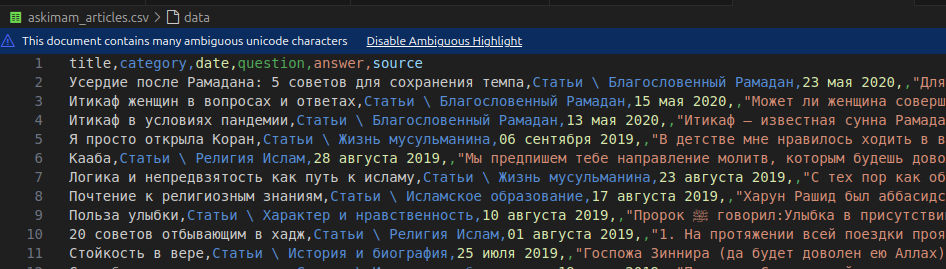
\includegraphics[width=0.9\linewidth]{image.png}
%     \caption{Parsing of askimam website}
%     \label{fig:enter-label}
% \end{figure}
% then describe each step in the appropriate section

% Describe problems that we need to overcome

% Short recap of the whole chapter




% WHAT WE DID TO ANSWER THE RESEARCH QUESTION
% We collaborated with an employee of Darul-Ifta in Tatarstan as our customer and domain expert. As the first stage, we conducted requirements elicitation. We then delivered a simple MVP  for the customer to use as part of our requirements engineering process.

% SYSTEM EVALUATION: HOW WE MEASURED THE RESULTS
% CLASSIFICATION - measure correctness
% AUTOMATIC PROCESSING - measure quality of answers
% HUMAN AUGMENTATION - how fast and satisfied

%  SYSTEM-AS-IS
% SYSTEM-TO-BE

% \subsection{Conclusion}

% Communicated with Dar-ul-Ifta Tatarstan, we decided to create a LLM-based agent system that will make the process of answering questions more efficient preserving authenticity. To implement it, firstly we collected, prepared, and analyzed the data, then, iteratively implemented the system, adjusting it based on the customer's feedback.
